\documentclass[11pt, oneside]{article}   	% use "amsart" instead of "article" for AMSLaTeX format
\usepackage{geometry}                		% See geometry.pdf to learn the layout options. There are lots.
\geometry{letterpaper}                   		% ... or a4paper or a5paper or ... 
%\geometry{landscape}                		% Activate for for rotated page geometry
\usepackage[parfill]{parskip}    		% Activate to begin paragraphs with an empty line rather than an indent
\usepackage{graphicx}				% Use pdf, png, jpg, or eps� with pdflatex; use eps in DVI mode
								% TeX will automatically convert eps --> pdf in pdflatex		
\usepackage{amssymb}
\usepackage{graphicx}
\usepackage{natbib}
\usepackage[nottoc,numbib]{tocbibind}
\usepackage{eqnarray}
\usepackage{setspace}
\usepackage{amsmath}

\usepackage{tikz}
\usetikzlibrary{shapes,arrows}

\onehalfspacing
\newcommand{\unit}[1]{\ensuremath{\, \mathrm{#1}}}


\title{MIT M.Eng. Thesis Proposal \\\ \textbf{Analyzing Motion in the Cochlea}}
\author{Logan Williams \\ \emph{Advisor: Prof. Dennis M. Freeman, Micromechanics Group, RLE}}

\begin{document}
\maketitle

\tableofcontents

\section{Introduction}

The mammilian cochlea is capable of remarkable sensory perception. It can distinguish motions as small as the radius of a hydrogen atom and discriminate between up to 30 frequencies within a single semitone. \cite{ghafarri} However, the mechanics of motion in the inner ear remain poorly understood. The Micromechanics Group at RLE is  analyzing motion in the cochlea in order to more fully understand what gives rise to these remarkable sensory abilities.

\begin{figure}[h!]
  \centering
    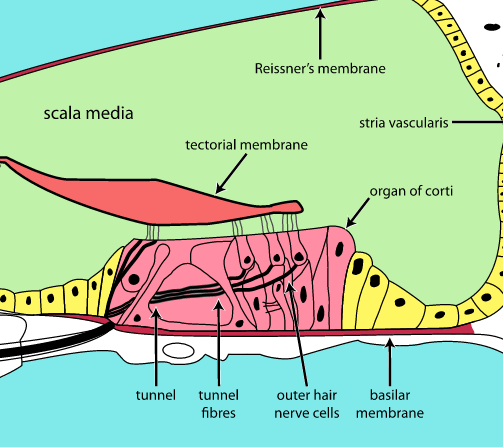
\includegraphics[width=0.8\textwidth]{images/cochlea.png}
      \caption{A schematic of tissues in the cochlea.}
      \label{fig:cochlea}
\end{figure}

A tissue of particular interest in the cochlea is the tectorial membrane, which is in direct contact with the hair cells, as shown in Figure \ref{fig:cochlea}. This tissue has some interesting mechanical properties, and its position in relation to the sensory cells suggests it could play in active role in motion amplification or in frequency discrimination. However, as it is almost entirely water, it is very difficult to image with conventional imaging techniques.

One successful technique for imaging these tissues, and understanding how they move under a given acoustic stimulus, has been doppler optical coherence microscopy, or DOCM. The Micromechancis group has been using this technique since 2006, with a system developed by former student Stanley Hong. \cite{hong}

This M. Eng. thesis will concentrate on creating a more modern, fiber based DOCM system for cochlear imaging.  Currently, due to the size and fixedness of the existing OCT system, aligning the optics with the biological sample is a time consuming process that can take over four hours. The fiber based OCT system will be smaller, and have a flexible fiber output. This will make it significantly easier to align the optics with the sample to be imaged. Furthermore, a fiber based OCT system would allow for complete water immersion of the optical system, resulting in less scattering loss and better signal characteristics.

\subsection{Title}

The working title for this M. Eng. thesis is ``Design, implementation, and applications of a fiber optic doppler optical coherence microscopy system for cochlear imaging.''

\section{The Fiber Optic DOCM System}

Optical coherence tomography, or OCT is a technique for inside scattering media, such as biological tissue. By utilizing the interference properties of broadband light sources, and the fact that near infrared light that can penetrate biological tissues, OCT is capable of imaging tissues deeper and with finer resolution than conventional technologies. When performed with a high NA lens to achieve fine transverse resolution as well, this technique is referred to as optical coherence microscopy, or OCM.

\subsection{Principle of operation and mathematical background}

\begin{figure}[h!]
  \centering
    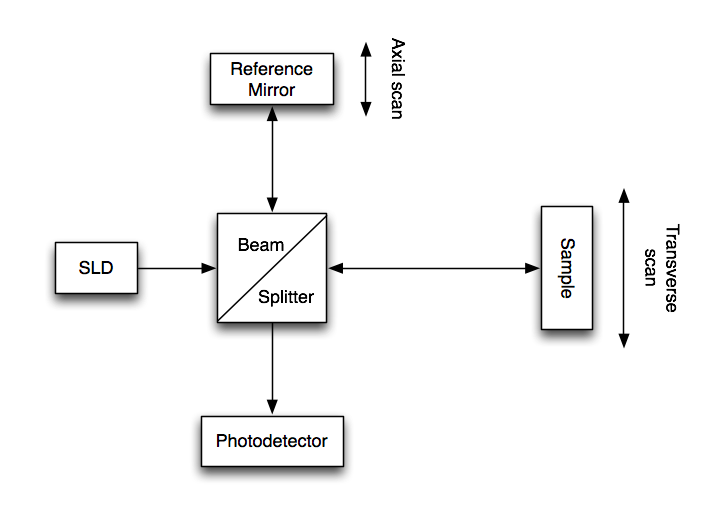
\includegraphics[width=0.8\textwidth]{images/basic_oct.png}
      \caption{A schematic of a basic OCT system.}
\end{figure}


OCT functions by utilizing the principle of the Michelson interferometer, as shown in Figure 1. Light is split in to two beams. One is reflected from a mirror, the other is scattered from a biological sample. The light is then recombined and the intensity measured by a photodetector. When the optical path lengths of the two beams are closely matched, and interference pattern may be observed. By using temporally incoherent (broadband) light, the interference pattern is capable of absolute localization.

The electric field from a temporally incoherent source can be modeled accurately as a wide-sense stationary random process with a certain power spectral density. \cite{Bouma} In the case where the scattering sample is replaced by a reflecting mirror, the mathematical analysis may be simplified greatly by assuming that two time delayed versions of this processes are being interfered. From this, we show that interference is the same as autocorrelation, and make use of the Wiener-Khinchin theorem. This derivation follows closely that of Fercher et. al. \cite{fercher}

The intensity of light with analytic (complex) amplitude $V(t)$ is defined as:

\begin{equation}
I(t) = V^*(t)V(t)
\end{equation}

In an OCT system, the light from a reference path is combined with the light from a sample path after some delay. We may express this as:

\begin{equation}
V_D(t; \Delta t) = V_S(t) + V_R(t + \Delta t)
\end{equation}

Of course, since measuring instantaneous electric field amplitude is impossible, we are interested in ensemble averages of intensity. This gives the following result, where $\Gamma_{XY}$ represents the cross correlation between two random processes $X$ and $Y$.

\begin{equation}
\begin{aligned}
\bar{I}_E(\Delta t) & =  \langle I_E(t; \Delta t) \rangle \\
& =  \langle V^*_E(t; \Delta t) V_E(t; \Delta t) \rangle \\
& =  \langle I_S(t) \rangle + \langle I_R(t) \rangle + 2 \Re \{\Gamma_{SR} (\Delta t) \}
\end{aligned}
\end{equation}

$\Delta t$ is proportional to the path length difference between the two beams, $\Delta t = \Delta z / c$. When both sample and reference paths are illuminated from the same light source, the cross correlation function above simplifies into an autocorrelation function of the light source. From here, the Wiener-Khinchin theorem can be applied, which states that the autocorrelation function of a wide-sense stationary random process is related to the process power spectral density by a Fourier transform.

\begin{equation}
\Gamma_{XX}(\tau) = 2 \int_{0}^\infty S_{XX}(f) \exp(2 \pi j \tau f) \,df
\end{equation}

Therefore, the axial resolution in an OCT system is limited by the spectral properties of the light source. Given a source of center wavelength $\lambda_0$ and bandwidth $\Delta \lambda$, if we assume a Gaussian PSD, we may find the width of the autocorrelation function, and therefore the axial resolution. \cite{fercher}

\begin{equation} \label{eq:ares}
\delta_z = l_c = \frac{2 \ln{2}}{\pi} \frac{\lambda_0^2}{\Delta \lambda}
\end{equation}

This however, is just the envelope of the autocorrelation function. It is also modulated by a carrier, with a  frequency dependent on the wavelength of the light source, $\lambda_0$, and the speed of the scan, $v_s$. \cite{fercher}

\begin{equation} \label{eq:carrier}
f_{mod} = 4 \pi v_s / \lambda_0
\end{equation}

The transverse resolution is the standard diffraction limit for a lens. \cite{hecht}

\begin{equation} \label{eq:tres}
\delta_x = 0.61 \frac{\lambda}{NA}
\end{equation}

\subsection{Measuring motion}

There are several methods of measuring motion of samples using optical coherence tomography. The method used by the existing DOCM system in the Micromechanics Group is based on acousto-optic modulators, or AOMs. AOMs are capable of changing the relative path length of light in response to an electrical stimulus, by creating acoustic  waves within a crystal.

\begin{figure}[h!]
\centering
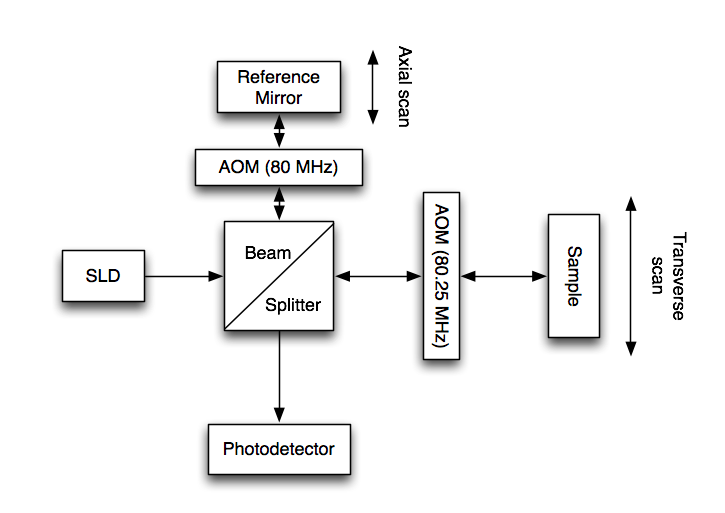
\includegraphics[width=0.8\textwidth]{images/oct_with_aoms.png}
\caption{An OCT system with AOMs in the light paths.}
 \label{fig:aom}
\end{figure}

In the configuration shown in Figure \ref{fig:aom}, the time-varying path length differences create a beat frequency in the measured light intensity at double the difference frequency (in this case, 500 KHz). Any motion of the sample will be multiplied by this carrier frequency, creating side bands around 500 KHz in the measured intensity. The amplitude and phase of motion can be found by analyzing these side bands. \cite{hong}

\subsection{Prior work}

During the 2012-2013 academic year, I worked under Professor Freeman to began implementing the planned Fiber Optic DOCM system. A schematic of this system is shown in Figure \ref{fig:actual}.

\begin{figure}[h!] 
  \centering
    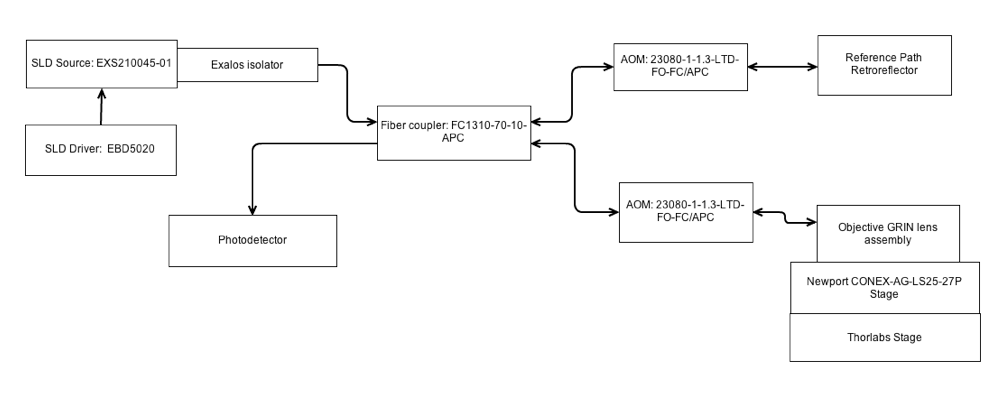
\includegraphics[width=\textwidth]{images/oct_with_part_numbers.png}
      \caption{A schematic of the actual FO-DOCM system.}
      \label{fig:actual}
\end{figure}

This system uses an Exalos super-luminescent diode as a light source ($\lambda_0 = 1310 \unit{nm}$, $\Delta \lambda = 100 \unit{nm}$). It uses a broadband fiber optic coupler to split the beams and a New Focus 2117 photodiode as a detector. The objective lens for the sample path is a Thorlabs GRIN assembly with a working distance of approximately 1.9 mm, while the lens for the reference path is a Thorlabs fiber coupled collimator ($f = 8.84 \unit{mm}$). Two fiber coupled AOMs from Gooch \& Housego will perform the heterodyning ($f_{res} = 80 \unit{MHz}$) but have not yet been integrated into the system. The objective lens is mounted on a Newport CONEX-AG piezo stage to perform axial scanning. The specifics of this stage apparatus and the transverse scanning apparatus have yet to be designed. The SLD is driven by an Exalos constant-current SLD driver. The AOM drive signals (80 and 80.25 MHz) are generated by a 1 GSPS digital frequency synthesizer.

The theoretical maximum resolution for this system is shown in Table 1, from equations \ref{eq:ares} and \ref{eq:tres}.

\begin{table}[h!]
\centering

\begin{tabular}{r  c  c}
 & \textbf{Axial} & \textbf{Transverse} \\
\noalign{\smallskip}
\textbf{Air} & $7.57 \unit{\mu m}$ & $1.74 \unit{\mu m}$ \\
\noalign{\smallskip}
\textbf{Immersion} & $4.73 \unit{nm}$ & $1.09 \unit{\mu m}$
\end{tabular}

\caption{Theoretical maximum resolution for the FO-DOCM system}
\end{table}

\subsubsection{Known issues}

Preliminary results on this system indicate significant debugging work remains. While interference fringes have been observed, the signal to noise ratio is several orders of magnitude lower than as designed. However, the measured FWHM of the interference fringes was approximately 9.2 $\mu$m, promisingly close to the predicted 7.57 $\mu$m.

\subsection{Planned work}

Planned work will focus on further implementing debugging, characterizing, and testing applications of the FO-DOCM system. In addition to the known issues and unconfigured components mentioned above, several areas require significant development.

\subsubsection{Signal processing and scan control}

Software will be developed to perform signal processing on the captured interference signal, and automate the control of X-Z scanning. The signal processing tool chain for capturing a standard OCT image is  shown in Figure 3. This chain is applied once for every axial scan (Z), and is repeated while translating the sample in X  to produce a two dimensional image.

% Define block styles
\tikzstyle{decision} = [diamond, draw, fill=blue!20, 
    text width=4.5em, text badly centered, node distance=3cm, inner sep=0pt]
\tikzstyle{block} = [rectangle, draw, fill=blue!20, 
    text width=6em, text centered, rounded corners, minimum height=4em]
\tikzstyle{line} = [draw, -latex']
\tikzstyle{cloud} = [draw, ellipse,fill=red!20, node distance=3cm,
    minimum height=2em]
    
\begin{figure}[h!]
  \centering
\begin{tikzpicture}[node distance = 2cm, auto]
    % Place nodes
    \node [block] (bpf) {band pass filter};
    \node [block, left of=bpf, node distance=3cm] (pd) {photodiode};
    \node [block, right of=bpf, node distance=3cm] (demod) {demodulator/ envelope follower};
    % Draw edges
    \path [line] (bpf) -- (demod);
    \path [line] (pd) -- (bpf);
\end{tikzpicture}
\caption{Basic OCT signal processing chain. The bandpass filter is centered around the carrier frequency from equation \ref{eq:carrier}. The demodulator either can be as straightforward as an envelope follower or a Hilbert transform based analytic continuation.}
\end{figure}

The signal processing software will also be able to process and analyze heterodyned doppler signals. This process is distinct from the above in that no scanning is performed, and more data must be collected for one data point. Because the heterodyne signal (with an acoustic frequency of $f$) is $500 \pm f$ KHz, a sampling rate of $>1$ MSPS is required. 

\begin{figure}[h!]
  \centering
\begin{tikzpicture}[node distance = 2cm, auto]
    % Place nodes
    \node [block] (bpf) {band pass filter};
    \node [block, left of=bpf, node distance=3cm] (pd) {photodiode};
    \node [block, right of=bpf, node distance=3cm] (demod) {hilbert transform envelope follower};
    \node [block, right of=demod, node distance=3cm] (fft) {sine fitter (least squares)};
     \node [block, below of=demod, node distance=2cm] (sine) {acoustic stimulus signal};
    % Draw edges
    \path [line] (bpf) -- (demod);
    \path [line] (pd) -- (bpf);
    \path [line] (sine) -- (fft);
    \path [line] (demod) -- (fft);
\end{tikzpicture}
\caption{Basic doppler OCT signal processing chain.}
\end{figure}

By comparing the fitted sine wave to the stimulus signal, the phase and amplitude of the acoustically induced motion may be determined.

\subsubsection{Alignment with sample and scanning}

An apparatus needs to be developed to assist the initial alignment of the objective GRIN lens with the sample tissues. This apparatus needs to be tested in experimental environments and evaluated primarily for ease of use.

One possibility is that by mounting the GRIN lens fiber at an angle with respect to vertical, the system could be placed beneath a small magnifying microscope. By coupling visible light into the fiber (the visible light would no longer be transmitted a single mode through the fiber, but as the light is used for visual alignment only, this is not an issue), the location of focus can be easily found.

A transverse scanning stage also remains to be built, and will likely depend on the specifics of the design of the alignment mechanism. The transverse scanning apparatus will either translate the GRIN lens while keeping the biological sample stationary, or translate the biological sample directly.

\subsubsection{Device characterization}

The resolution limits and properties of the FO-DOCM system will be characterized, quantized, and compared with the theoretical values. The noise floor of heterodyned motion detection will also be measured, and compared with the older DOCM system.

\section{Applications}

While the M.Eng. thesis will primarily focus on the development and properties of the FO-DOCM device, relevant applications will also be explored.

\subsection{Motion and resonance in the cochlea}

The most obvious application of the new FO-DOCM apparatus is as a direct replacement for the current DOCM system in the Micromechanics Group. As was mentioned in the introduction, the current system has several deficiencies, which the fiber system is designed to address. 

The experiments currently being performed with this system involve \emph{in vivo} experiments on gerbil and guinea pig cochleas. With an applied auditory stimulus, the relative amplitude and phase of motion of different parts of the cochlea are measured. The flexibility of the fiber optic system should make working \emph{in vivo} significantly less time consuming by easing the setup and alignment process. The degree to which it does so will be evaluated, and improvements and modifications to the system will be made as necessary to support further applications in this area.

\subsection{Polarization sensitive OCT}

Previous researchers have had success with using polarization sensitive microscopy to image cochlear tissues. \cite{kalwani} Polarization sensitive OCT could be capable of imaging the tectorial membrane and other cochlear tissues with greater contrast than conventional OCT.

While the tectorial membrane is 97\% water, by dry mass it is 50\% collagen, a protein that typically has enhanced contrast in polarization sensitive imaging due to its periodic structure. Also due partially to the regular organization of collagen fibers, the TM is mechanically anisotropic. \cite{freemandynamic} Imaging the TM in a phase sensitive way could visually highlight this anisotropy.

This application of a DOCM system would be novel for cochlear imaging, but more background research needs to be done to evaluate feasibility. If feasible, this new imaging technique could be used with either of the existing DOCM systems in the Micromechanics Group.

\section{Timeline}

The following is an approximate timeline for work on this thesis. The overall goal will be to create a functional DOCM imaging system and collect enough high quality data such that an academic journal article could be written.

\begin{description}
\item[September -- October] Device characterization and benchtop testing.
\item[November -- December] Alignment apparatus testing. Using the system with biological samples.
\item[January -- February] Evaluating potential applications and collecting data.
\item[March -- April] Collecting data. Thesis/article writing.
\item[May]  Wrap up, or possibly continue/finish work over the summer, as needed.
\end{description}

\bibliographystyle{plain}

\bibliography{proposal}


\end{document}  